\documentclass[a4paper, 11pt]{article}
\renewcommand{\baselinestretch}{1.1}
\usepackage{comment}
\usepackage{lipsum}
\usepackage{fullpage}
\usepackage[a4paper, total={7in, 10in}]{geometry}
\usepackage{amsmath}
\usepackage[utf8]{inputenc}
\usepackage[russian]{babel}
\usepackage{amssymb,amsthm}

\newtheorem{theorem}{Theorem}
\newtheorem{corollary}{Corollary}
\usepackage{graphicx}
\usepackage{tikz}
\usetikzlibrary{arrows}
\usepackage{verbatim}
\usepackage{xcolor}
\usepackage{mdframed}
\usepackage[shortlabels]{enumitem}
\usepackage{indentfirst}
\setlength{\parindent}{0cm}
\usepackage{hyperref}
\usepackage{float}

\usepackage{setspace}
\setlength{\parindent}{20pt}
\setlength{\parskip}{4pt}

\graphicspath{{./images/}}

\newcommand{\beq}{\begin{equation}}
\newcommand{\eeq}{\end{equation}}

\begin{document}
\section{Общая структура работы.}

Модель KGD: трещина с прямоугольным вертикальным сечением; применима в случаях, когда высота трещины много больше её длины; допущение о плоской деформации в горизонтальной плоскости;
\\

Модель PKN: трещина с эллиптическим вертикальным сечением; применима в случаях, когда полудлина трещины много больше её высоты; допущение о плоской деформации в вертикальной плоскости;
\\

\section{Важные источники.}

1) Ткаченко Д.Р. Анализ влияния режима работы нагнетательной скважины на рост трещны автоГРП.

2) Hagoort J. Waterflood-induced hydraulic fracturing. PhD. Thesis, Delft Technical Univeёrsity, 1981 (моделирование трещин на нагнетательных скважинах; для трещины KGD получена формула для давления распространения трещины)

3) Hagoort J., Weatherill B.D. and Settari A. Modeling the propagation of waterflood-induced hydraulic fractures. (объединили аналитическую модель трещины с численной моделью пласта и изучили скорость распространения трещины; сделан вывод, что обычная модель Картера для одномерных утечек, перпендикулярных трещине, не всегла верна; здесь показано, что в бесконечном пласте при любой скорости распространения трещины её длина будет пропорциональна квадратному корню времени, различия будут только в коэффициентах)

4) Koning E.J.L. Fractured water-injection wells. Analytical modelling of fracture propagation.

5) Кабанова П.К. Моделирование давления инициации трещины гидроразрыва пласта на нагнетательной скважине в пороупругой постановке (поведение линейной изотропной пороупругой среды)

6) T.K. Perkins, L.R. Kern. Widths of hydraulic fractures

7) R.P. Nordgren. Propagation of vertical hydraulic fractures

8) Тримонова М., Дубиня Н., Основные закономерности развития трещины автоГРП

9) Perkins T.K., Gonzalez, J.A. The effect of thermo-elastic stresses on injection well fracturing ()

10) Gringarten A. C., Ramey H. J., Raghavan R. Unsteady-State Pressure Distributions Created by a Well With a Single Infinite-Conductivity Vertical Fracture. Society of Petroleum Engineers (аналитическое выражение для нахождения давления с постоянной скоростью расхода в стационарной трещине бесконечной проводимости)

11)
\\

\section{Дополнительные источники.}

1) Economides. Unified Fracture Design. Bridging the gap between theory and practice.

2) Логвинюк А.В. Комплексный анализ и моделирование разработки Приобского месторождения для оптимизации системы поддержания пластового давления

3) Старобинский Е.Б. Разработка модели распространения планарной трещины ГРП в слоистой среде

4) Дегтерев Д.А. Интегральные преобразования в планарной модели трещины гидроразрыва пласта

5) Краева С.О. Моделирование переноса и оседания проппанта в трещине ГРП

6) Барсуков С.С. Задача экспресс-оценки корректности моделирования трещины ГРП на примере постановки planar3D.

7) Perkins T. K., Kern L. R. Widths of Hydraulic Fractures

8) Koning E.J.L. Poro- and thermo-elastic rock stresses around a wellbore

9) 
\\


\section{Общие заметки.}

1) Если скорость давления, проходящего через пласт, имеет порядок скорости распространения трещины, распределение утечек будет двумерным в плоскости пласта. Т.е. одномерная модель утечек (модель Картера) не работает.

2) Предположение о малости полудлины трещины по сравнению с толщиной пласта (модель KGD).

3) Модель Картера перестаёт быть верной, когда скорость распространения трещины становится меньше скорости пластового давления.
Возможные режимы утечек: линейный 1D режим (Картер), эллиптический 2D режим (Грингартен), радиальный режим.

4) Повлиять на состояние напряжения в пласте может изменение температуры и давления в нём.
Когда пласт охлаждается, то порода начинает сжиматься и, следовательно, происходит термоупругое уменьшение горизонтальных напряжений пласта.
Поэтому опасно закачивать холодную воду в пласт (неконтроллируемый рост трещин автоГРП).
Изменения горизонтального напряжения в пласте зависит от соотношения высоты трещины и глубины проникновения давления / фронта температур.

5) Насыщение пласта водой по мере закачки может сдерживать рост трещины за счёт эффектов пороупругости.

6) Для случая нулевой утечки: по модели PKN эффективное давление увеличивается во времени, а по модели KGD и радиальной -- уменьшается во времени.
Из постулатов модели KGD (и в радиальной тоже) вытекает, что когда размеры трещины становятся очень большими, требуются очень малые эффективные давления для поддержания определенной ширины.
Хотя это является следствием теории линейной упругости и того способа, как применено допущение о плоской деформации, в целом это приводит к абсурдным результатам.
Можно с уверенностью сказать, что модель PKN лучше описывает физику процесса гидроразрыва, чем две другие модели.

7)
\\

\section{Вопросы.}

1) Важно ли предположение о малости полудлины трещины (по сравнению с высотой пласта) в модели KGD для возможности рассмотрения плоско-деформированной задачи?
Вроде это не связано.
Предположение о малости высоты или полудлины равносильно тому, используем ли двухмерный или одномерный поток жидкости по трещине.
В KGD плоская деформация в горизонтальной плоскости, а в PKN -- в вертикальной.

2) 

3)

\newpage
\section{Перевод статьи Нордгрена (Распространение вертикальной трещины гидроразрыва пласта)}

\subsection{Реферат}
В данной статье рассматривается распространение трещин гидроразрыва с ограниченной высотой и эллиптическим вертикальным сечением с учётом эффекта утечек жидкости.
Представлены численные и асимптотические приближённые решения в безразмерной форме, которые дают длину и ширину трещины в любой момент времени и при любом наборе физических параметров.
Ознакомление с безразмерными результатами и приближёнными решениями должно быть полезно при разработке дизайна ГРП.

\subsection{Введение}
Теория и практика гидроразрыва пласта были рассмотрены Howard-ом и Fast-ом.
Поэтому мы ограничим обсуждение предыдущих исследований только темами, которые имеют отношение к текущему исследованию распространения вертикальных трещин.

Важным теоретическим результатом является формула Картера для трещины постоянной ширины, образованной закачкой жидкости с постоянным расходом, с учётом потери жидкости в пласт.
Для вертикальной трещины постоянной высоты формула Картера даёт длину трещины как функцию времени.
В общем случае предположение Картера о постоянной ширине трещины не реалистично.
Однако на больших временах ошибка, вызванная этим предположением, становится несущественной, так как доминируют утечки жидкости в пласт.

Ширина вертикальной трещины впервые была исследована Христиановичем и Желтовым в предположении, что ширина не изменяется в вертикальном направлении.
Таким образом, в горизонтальных плоскостях преобладает состояние плоской деформации и ширина может быть определена как решение плоской задачи упругости.
Приближённое решение найдено в [3] при пренебрежении утечками жидкости, изменением объёма трещины и изменением давления вдоль трещины.
Длина трещины определена из условия конечных напряжений на кончике трещины.
Baron et al. [4] и Гиртсма и деКлерк [5] включили эффект утечек жидкости к подходу [3].
Гиртсма и деКлерк дают простые приближённые формулы для длины и ширины трещины.

Другой подход к определению ширины трещины был использован Перкинсом и Керном.
Они рассмотрели трещину постоянной высоты в предположении плоской деформации в вертикальных плоскостях, перпендикулярных плоскости трещины.
Поперечное сечение трещины в таком предположении получается эллиптическим, а максимальная ширина уменьшается вдоль трещины по простой формуле, содержащей длину трещины.
При выводе этой формулы [6] использовались допущения отсутствия утечек и неизменности объёма трещины в уравнении сплошности, и длина трещины не определяется.
В последующих приложениях [7] предполагалась "<разумная"> длина трещины.
Формула Картера для длины трещины и формула Перкинса и Керна для ширины трещины были процитированы Howard-ом и Fast-ом, и считается, что совместное использование этих двух формул является обычной практикой.

В настоящем теоретическом исследовании рассматривается трещина ограниченной высоты типа, изученного Перкинсом и Керном.
Однако мы включаем эффекты потери жидкости и изменения объёма трещины в уравнение сплошности.
Следовательно, длина трещины определяется как часть решения.
Общие результаты по изменению ширины и длины трещины во времени получены в безразмерном виде численным методом.
Кроме того, выводятся асимптотические решения для больших и малых значений времени.
Решение для малого времени также является точным решением для случая отсутствия утечек жидкости в пласт.
Для больших значений времени наша асимптотическая формула для длины трещины идентична формуле Картера [2] для больших времён.
Наша формула для больших времён для ширины трещины отличается от формулы Перкинса и Керна [6] числовым коэффициентом, который меняется вдоль трещины.
В сравнении с нашей формулой эта формула [6] переоценивает ширину трещины около скважины на 12\% и на середине трещины -- на 24\%. 
На ранних временах формула Перкинса и Керна [6] для ширины трещины снова даёт хорошее приближение к нашему результату.
Однако наша формула для длины трещины отличается от формулы Картера [2], которая неприменима, так как пренебрегаемое в ней изменение ширины трещины важно на ранних временах (формула Картера выведена в предположении неизменности ширины трещины, но это изменение важно учитывать на ранних временах).

Результаты для ширины трещины, ограниченной по высоте, полученные здесь и в работе [6] отличаются от результатов для трещин, постоянных по высоте [3-5].
В частности наше решение для ширины на больших временах отличается от решения Гиртсмы и деКлерка коэффициентом, пропорциональным корню четвёртой степени из высоты трещины, делённому на длину трещины.
Это отличие может быть существенным в практических приложениях, и мы обсудим его далее.

В следующем разделе мы сформулируем задачу об ограниченных по высоте трещинах в духе работы [6].
Основные предположения обсуждаются более подробно.
Затем основные уравнения приводятся в безразмерную форму, пригодную для численного решения, которое выполняется в Приложении А.
В последнем разделе статьи даётся сравнение с предыдущими исследованиями и обсуждение применимости настоящих результатов.

\subsection{Формулировка задачи}

Рассмотрим вертикальную трещину, распространяющуюся по прямой от скважины (рис. \ref{fig:kgd-model-geometry}).
Как и в [6] предполагается, что вертикальная высота трещины ограничена постоянной величиной $h$ слоями устойчивой к разрушению породы.
Сопротивление разрушению может быть связано с более высоким горизонтальным тектоническим напряжением или более высокой прочностью на разрыв в породе, окружающей коллектор.

\begin{figure}[H]
\center
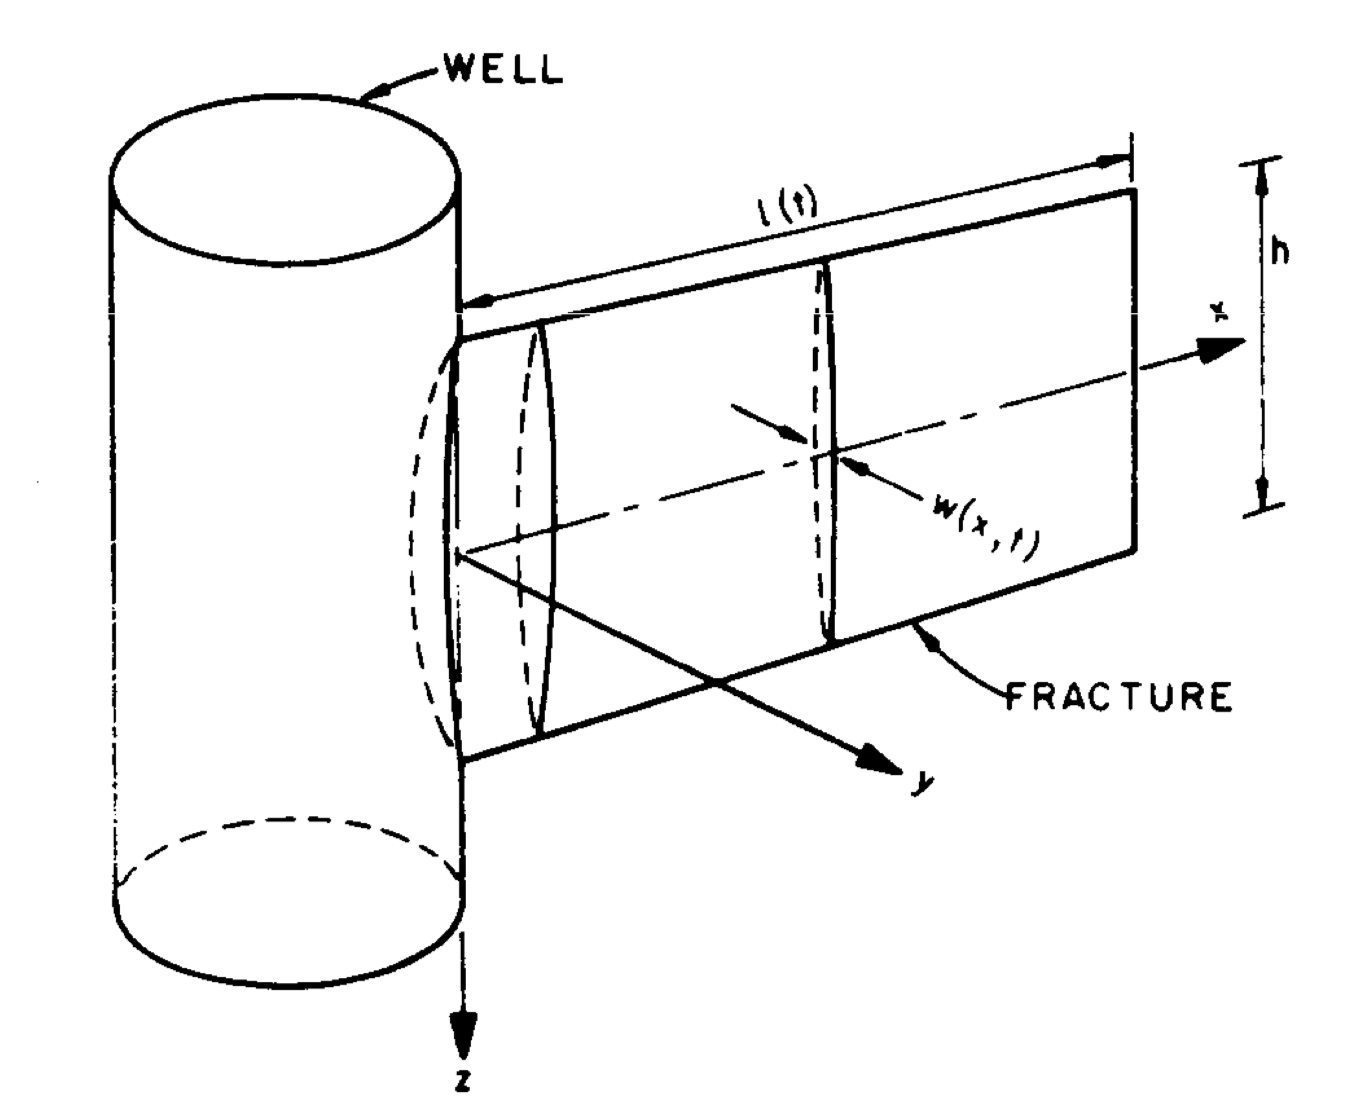
\includegraphics[width=0.5\textwidth]{fracture_geometry}
\caption{Геометрия трещины} 
\label{fig:kgd-model-geometry}  
\end{figure}

Пусть $x$, $y$, $z$ -- система прямоугольных декартовых координат с осью $x$ в направлении распространения трещины, осью $z$, параллельной оси скважины, и началом в забое (рис. \ref{fig:kgd-model-geometry}).
Таким образом, трещина лежит в плоскости $Oxz$ при $0\leqslant x\leqslant L$ и $|z|\leqslant \frac{1}{2}h$.

Следуя за [6], мы предполагаем, что трещину окружает изотропный однородный упругий материал.
Предположение об однородности может не полностью согласовываться с нашим более ранним предположением о том, что трещиностойкая порода ограничивает трещиноватый коллектор.
Однако на основе принципа Сен-Венана в теории упругости упругое поведение вблизи трещины контролируется в основном породой коллектором, и умеренно отличающаяся окружающая порода должна иметь небольшое влияние на ширину трещины.
Мы ограничиваем наше внимание стадией распространения трещины, когда её длина $L$ много больше высоты $h$, и все величины будут изменяться медленно по оси $x$ вдоль большей части трещины.
Это предположение будет проверено после того, как мы получим решение.
Ввиду ожидаемых медленных изменений величин вдоль оси $x$ в вертикальных плоскостях ($x=\textrm{const}$), перпендикулярных трещине, в некотором приближении преобладает состояние плоской деформации.

Перед гидроразрывом сжимающее напряжение ($S$), действует на плоскости, параллельные трещине в коллекторе.
Другие значения $S$ в породе, окружающей резервуар, опять же должны иметь пренебрежимо малый эффект.
Жидкость в трещине находится под давлением $S+\Delta p$ и мы пренебрегаем изменением $\Delta p$ вдоль координаты $z$, т.е. $\Delta p =\Delta p(x,t)$.
Тогда в соответствии с решением задачи о плоской деформации для трещины при постоянном давлении [8], вертикальное сечение трещины имеет форму эллипса и ширина $w(x,t)$ определяется выражением:
\beq\label{width}
w=
\begin{cases}
\dfrac{1-\nu}{G}\left(h^2-4z^2\right)^{1/2}\Delta p,\text{ если }|z|\leqslant\dfrac{1}{2}h,\\[10pt]
0,\text{ если }|z|\geqslant\dfrac{1}{2}h,
\end{cases}
\eeq
где $G$ и $\nu$ -- объёмный модуль сдвига и коэффициент Пуассона для пласта соответственно.
Решение с плоской деформацией не учитывает влияние изменение порового давления на упругую реакцию (упругое состояние породы), которое является небольшим эффектом в задачах разрушения.

Далее рассмотрим течение жидкости в трещине.
Уравнение неразрывности течения несжимаемой жидкости в трещинеможно записать в виде:
\beq\label{Continuity}
\frac{\partial q}{\partial x}+q_l+\frac{\partial A}{\partial t}=0,
\eeq
где $q(x,t)$ -- объёмный расход через поперечное сечение ($x=\textrm{const}$) трещины, $q_l(x,t)$ -- объёмная скорость утечек жидкости в пласт на единицу длины трещины и $A(x,t)$ -- площадь поперечного сечения трещины.

Мы предполагаем, что $q$ связан с градиентом давления классическим решением для ламинарного потока ньютоновской вязкой жидкости в эллиптической трубе с полуосями $\frac{1}{2}h$ и $\frac{1}{2}w_{max}$, где $h\gg w_{max}$, а именно
\beq\label{q_vs_gradient_p}
q=-\frac{\pi W^3h}{64\mu}\frac{\partial\Delta p}{\partial x},\,\,\,\,\,\,\,W=w_{max}
\eeq
где $\mu$ -- вязкость жидкости гидроразрыва. Диапазон применимости ламинарного потока обсуждался в [6].
Из формулы \eqref{width}:
\beq\label{Max_W}
W=w|_{z=0}=\frac{(1-\nu)h}{G}\Delta p
\eeq
и выражение \eqref{q_vs_gradient_p} перепишется в следующем виде:
\beq\label{q_vs_w}
q=-\frac{\pi G}{256(1-\nu)\mu}\frac{\partial}{\partial x}\left(W^4\right)
\eeq

Площадь поперечного сечения эллиптической трещины:
\beq\label{A_area}
A=\int\limits_{-h/2}^{h/2}w\,dz=\frac{\pi}{4}Wh
\eeq

Скорость утечек жидкости в пласт $q_l$ связана со скоростью утечек на единицу площади поверхности трещины следующим равенством:
\beq
q_l=2\int\limits_{-h/2}^{h/2}u_l\,dz,
\eeq
и если $u_l$ не зависит от $z$, то
\beq\label{leak-offs}
q_l=2hu_l
\eeq

Эксперименты [1, 11] показывают, что для многих жидкостей гидроразрыва скорость утечек можно принять в виде:
\beq\label{leak-off}
u_l=\frac{C}{\sqrt{t-\tau}},
\eeq
где $C$ -- коэффициент утечек жидкости и $\tau$ -- время начала течения.
Коэффициент $C$ зависит от различных параметров жидкости и пласта и обычно определяется экспериментально.
Для некоторых жидкостей формулу \eqref{leak-off} следует изменить, включив в неё так называемую "<скачкообразную утечку"> в момент времени $t=\tau$.
Установлено, что влияние скачкообразной утечки на длину трещины в целом невелико (см. приложение E).
Мы принимаем формулу \eqref{leak-off} в настоящей работе, хотя условия, при которых она была проверена экспериментально, строго не выполняются.
А именно разность между давлением в трещине $S+\Delta p$ и пластовым поровым давлением $p_f$, т.е.
\beq\label{pressures_difference}
S+\Delta p-p_f
\eeq
содержит $\Delta p$, которое меняется в зависимости от координаты $x$ и времени $t$.
В некоторых случаях $\Delta p\ll S-p_f$, так что предположение о постоянной разнице давлений должно привести к значимым результатам.
Более того, мы обнаружим, что $\Delta p$ медленно меняется в зависимости от $t$ и $x$ и использование среднего значения для $\Delta p$ в выражении \eqref{pressures_difference} может быть приемлемым.
Условие одномерности течения также строго не выполняется, хотя ввиду медленного изменения $\Delta p$ в зависимости от $x$ результирующая ошибка должна быть малой.
Теоретические уточнения в определении $q_l$ потребуют дополнительных экспериментальных исследований поведения фильтрационной корки под давлением, зависящим от времени.
Кроме того, рассмотрение двухфазного потока необходимо, если жидкость гидроразрыва существенно отличается от жидкости в порах пласта.

В скважине ($x=0$) необходимо задать граничное условие, включающее $q$ и $p$.
Это условие будет зависеть от зависимости $q(p)$ для насосного оборудования, используемого в процессе ГРП.
Здесь мы рассматриваем случай постоянной скорости притока:
\beq\label{gu1}
q(0,t)=q_i=\textrm{const}.
\eeq
В случае других граничных условий задача может быть решена численным методом, представленным в Приложении А.

Изначально трещина закрыта, т.е.
\beq\label{Initial_cond}
W(x,0)=0
\eeq
Более того, трещина остаётся закрытой при $x\geqslant L(t)$, т.е.
\beq\label{GU_1}
W(x,t)=0,\,\,\,\,\,x\geqslant L(t),
\eeq
где длина трещины $L(t)$ должна быть определена как часть решения.

После подстановки \eqref{q_vs_w}, \eqref{A_area}, \eqref{leak-offs} и \eqref{leak-off} в уравнение \eqref{Continuity}, получаем
\beq\label{Main_eq}
\frac{G}{64(1-\nu)\mu h}\frac{\partial^2}{\partial x^2}\left(W^4\right)=\frac{8C}{\pi\sqrt{t-\tau(x)}}+\frac{\partial W}{\partial t},\,\,\,\,\,\,\,0\leqslant x\leqslant L,\,\,\,\,\,\,\,t>0,
\eeq
где $\tau(x)$ -- время, когда трещина открылась в точке с координатой $x$, т.е.
\beq
\tau[L(t')]=t',\,\,\,\,\,\,\,\,0\leqslant t'\leqslant t
\eeq
Другими словами, $\tau(x)$ -- это функция, обратная к $L(t)$.

Подстановка формулы \eqref{q_vs_w} в граничное условие \eqref{gu1} даёт:
\beq\label{GU_2}
-\left[\frac{\partial}{\partial x}(W^4)\right]_{x=0}=\frac{256(1-\nu)\mu}{\pi G}q_i.
\eeq

Теперь нашей задачей является решение нелинейного дифференциального уравнения в частных производных \eqref{Main_eq} для раскрытия $W(x,t)$ при начальном условии \eqref{Initial_cond} и граничных условиях \eqref{GU_1} и \eqref{GU_2}.
Длину $L(t)$ тоже необходимо найти.

Чтобы свести к минимуму объём вычислений, удобно привести основные уравнения к безразмерному виду.
Таким образом, если мы введём $x=ax_{d}$, $L=aL_{d}$, $t=Bt_{d}$, $W=eW_d$, где
\beq\label{Dimensionless}
a=\pi\left[\frac{(1-\nu)\mu q_i^5}{256C^8Gh^4}\right]^{1/3},\,\,\,\,\,B=\pi^2\left[\frac{(1-\nu)\mu q_i^2}{32C^5Gh}\right]^{2/3},\,\,\,\,\,e=\left[\frac{16(1-\nu)\mu q_i^2}{C^2Gh}\right]^{1/3},
\eeq
то математическая постановка задачи перепишется в следующем виде:
\beq\label{FullTask}
\begin{cases}
\dfrac{\partial^2}{\partial x_d^2}(W_d^4)=\dfrac{1}{\sqrt{t_d-\tau_d(x)}}+\dfrac{\partial W_d}{\partial t_d},\\[15pt]
\left[\dfrac{\partial}{\partial x_d}(W_d^4)\right]_{x_d=0}=1,\\[15pt]
W(x_d,0)=0,\\[5pt]
W_d(x_d,t_d)=0\text{ для } x_d\geqslant L_d,\\[5pt]
\tau_d[L_d(t_d')]=t_d'\text{ для }0\leqslant t_d'\leqslant t_d.
\end{cases}
\eeq

Задача \eqref{FullTask} на $W_d(x_d,t_d)$ решена численно в Приложении A.


\subsection{Обсуждение результатов}

Результаты были получены тремя разными методами.
Численный метод из приложения A был применён к безразмерной задаче \eqref{FullTask}.
Зависимости длины трещины $L_d(t_d)$ и ширины трещины около скважины $W(0,t_d)$ от времени $t_d$ представлены на рис. \ref{fig:length-vs-time} и \ref{fig:width-at-well-vs-time}.

Приближённое решение в элементарных функциях выводится в приложении B при пренебрежении слагаемы $\frac{\partial A}{\partial t}$ в уравнении \eqref{Continuity}.
Это приближение справедливо на достаточно больших временах (как указано в приложении B) и подтверждается сравнением с численными результатами на рис. \ref{fig:length-vs-time} и \ref{fig:width-at-well-vs-time}.
При погрешности приближения менее 10\% при $t_d>1.0$.

\begin{figure}[H]
\center
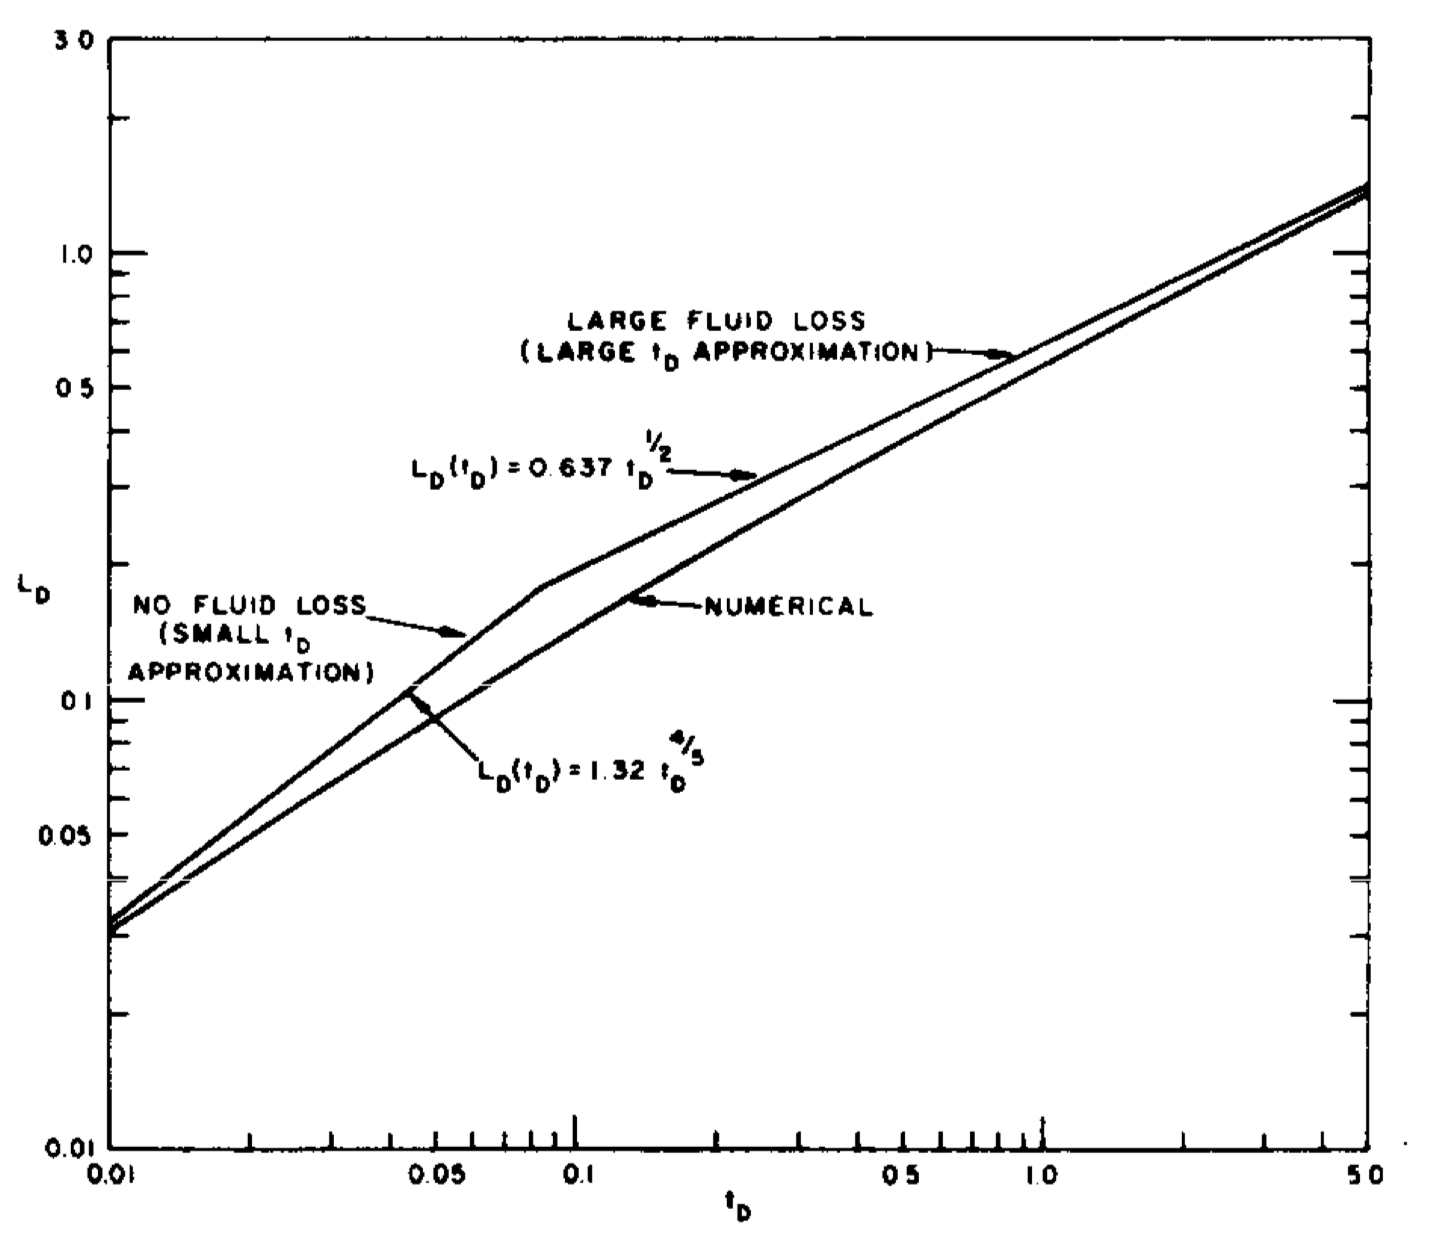
\includegraphics[width=0.5\textwidth]{length_vs_time}
\caption{Безразмерная длина трещины в зависимости от безразмерного времени} 
\label{fig:length-vs-time}  
\end{figure}


\begin{figure}[H]
\center
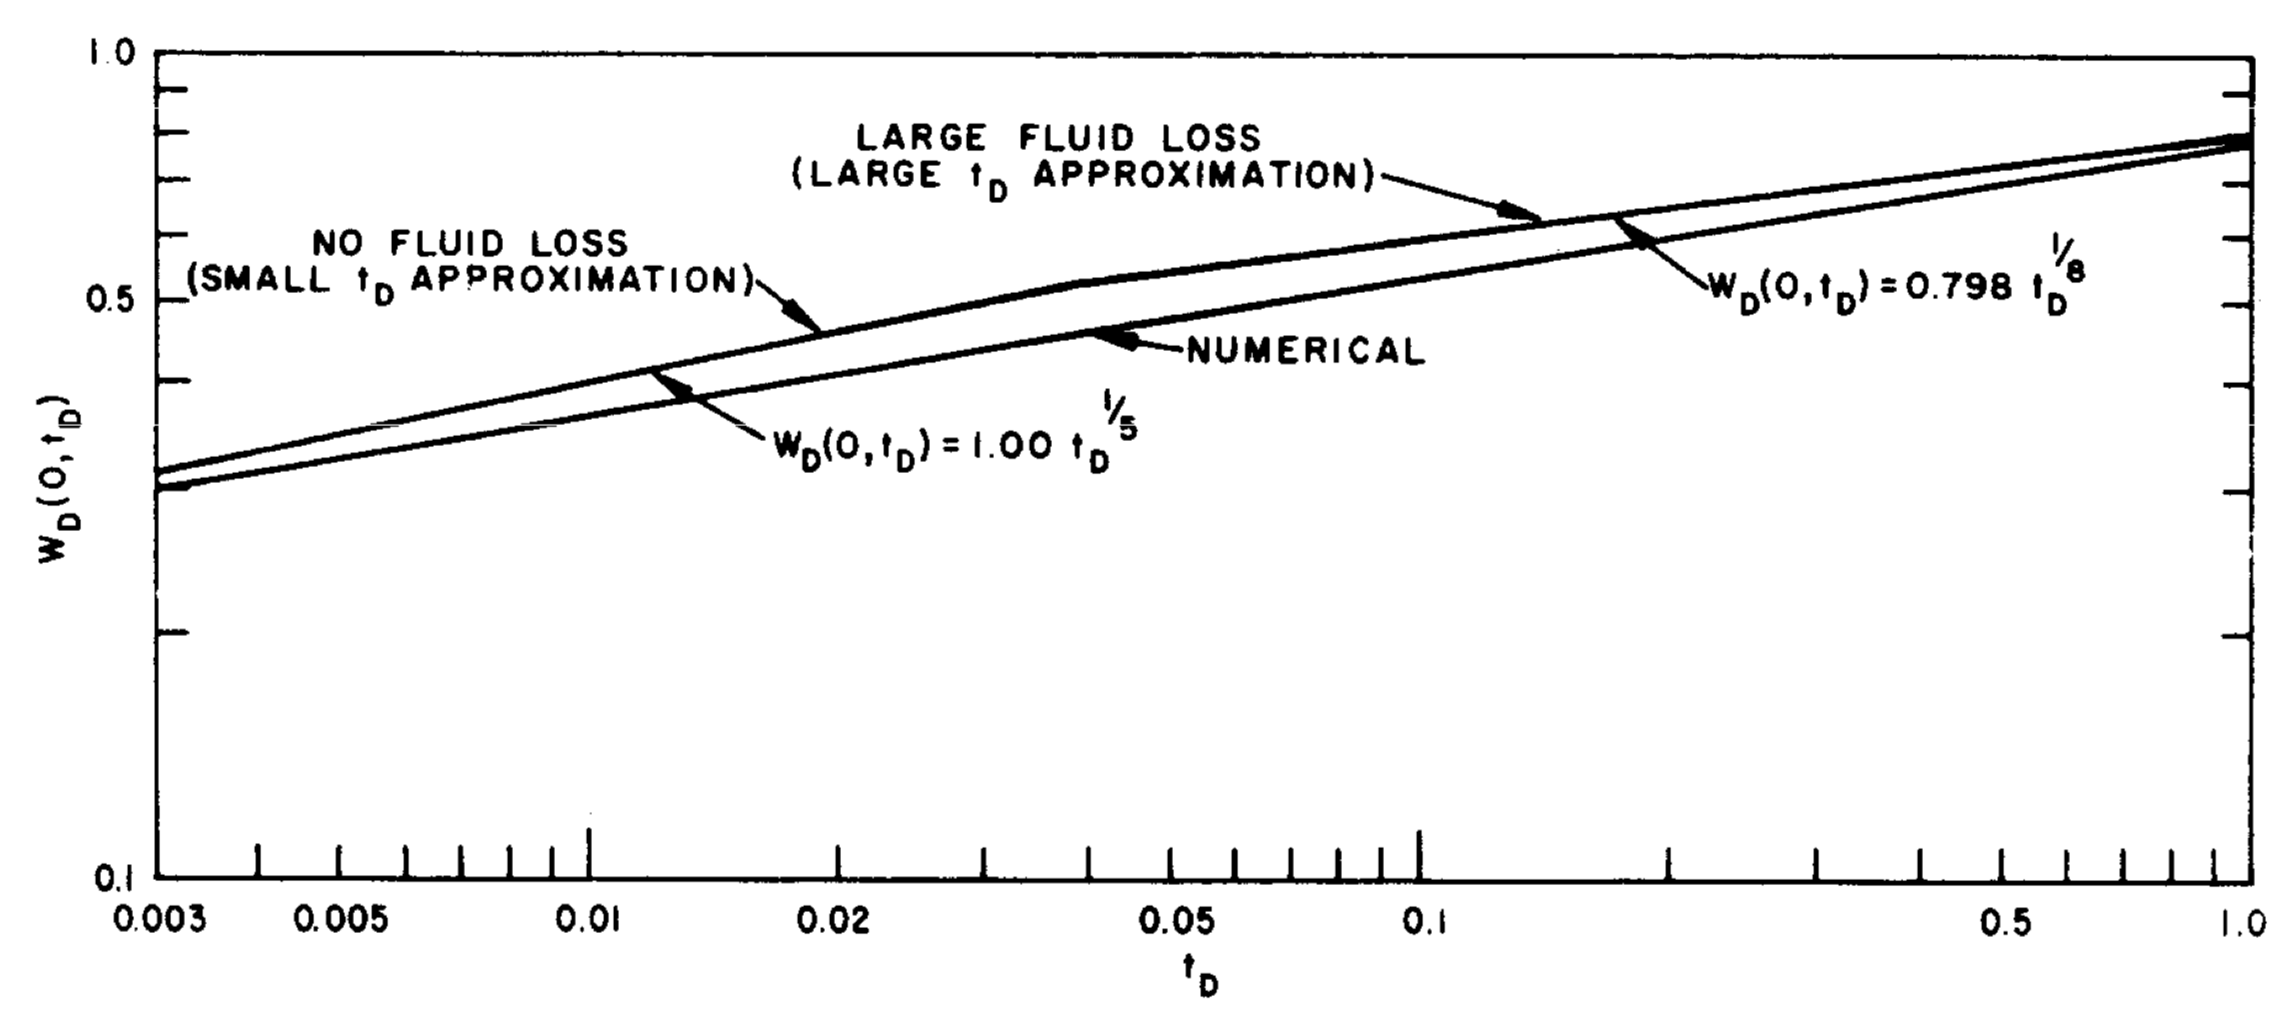
\includegraphics[width=0.8\textwidth]{maximum_width_at_well_vs_time}
\caption{Максимальная безразмерная ширина трещины около скважины в зависимости от безразмерного времени} 
\label{fig:width-at-well-vs-time}  
\end{figure}

Случай отсутствия утечек жидкости в пласт рассматривается в приложении C.
Преобразование подобия в сочетании с численным методом приложения A даёт решение для любого значения времени.
Результаты приложения C также представляют собой приближённое решение для случая потери жидкости из трещины за достаточно малое время.
По сравнению с численным решением на рис. \ref{fig:length-vs-time} и \ref{fig:width-at-well-vs-time} ошибка приближения составляет менее 10\% при $t_d<0.01$.
Кроме того, $t_d$ должно быть достаточно большим, чтобы выполнялось условие $L\gg h$, как обсуждается ниже.

На рис. \ref{fig:width-vs-distance-from-well} показано изменение максимальной ширины трещины вдоль её длины (по координате $x$) в безразмерной форме для приближённых решений Приложения B и Приложения C.
Эти две зависимости ширины трещины от координаты $x$ удивительно похожи.
Зависимость ширины от координаты $x$, полученная численным методом, лежит близко к зависимостям на рис. \ref{fig:width-vs-distance-from-well} и не показана.

\begin{figure}[H]
\center
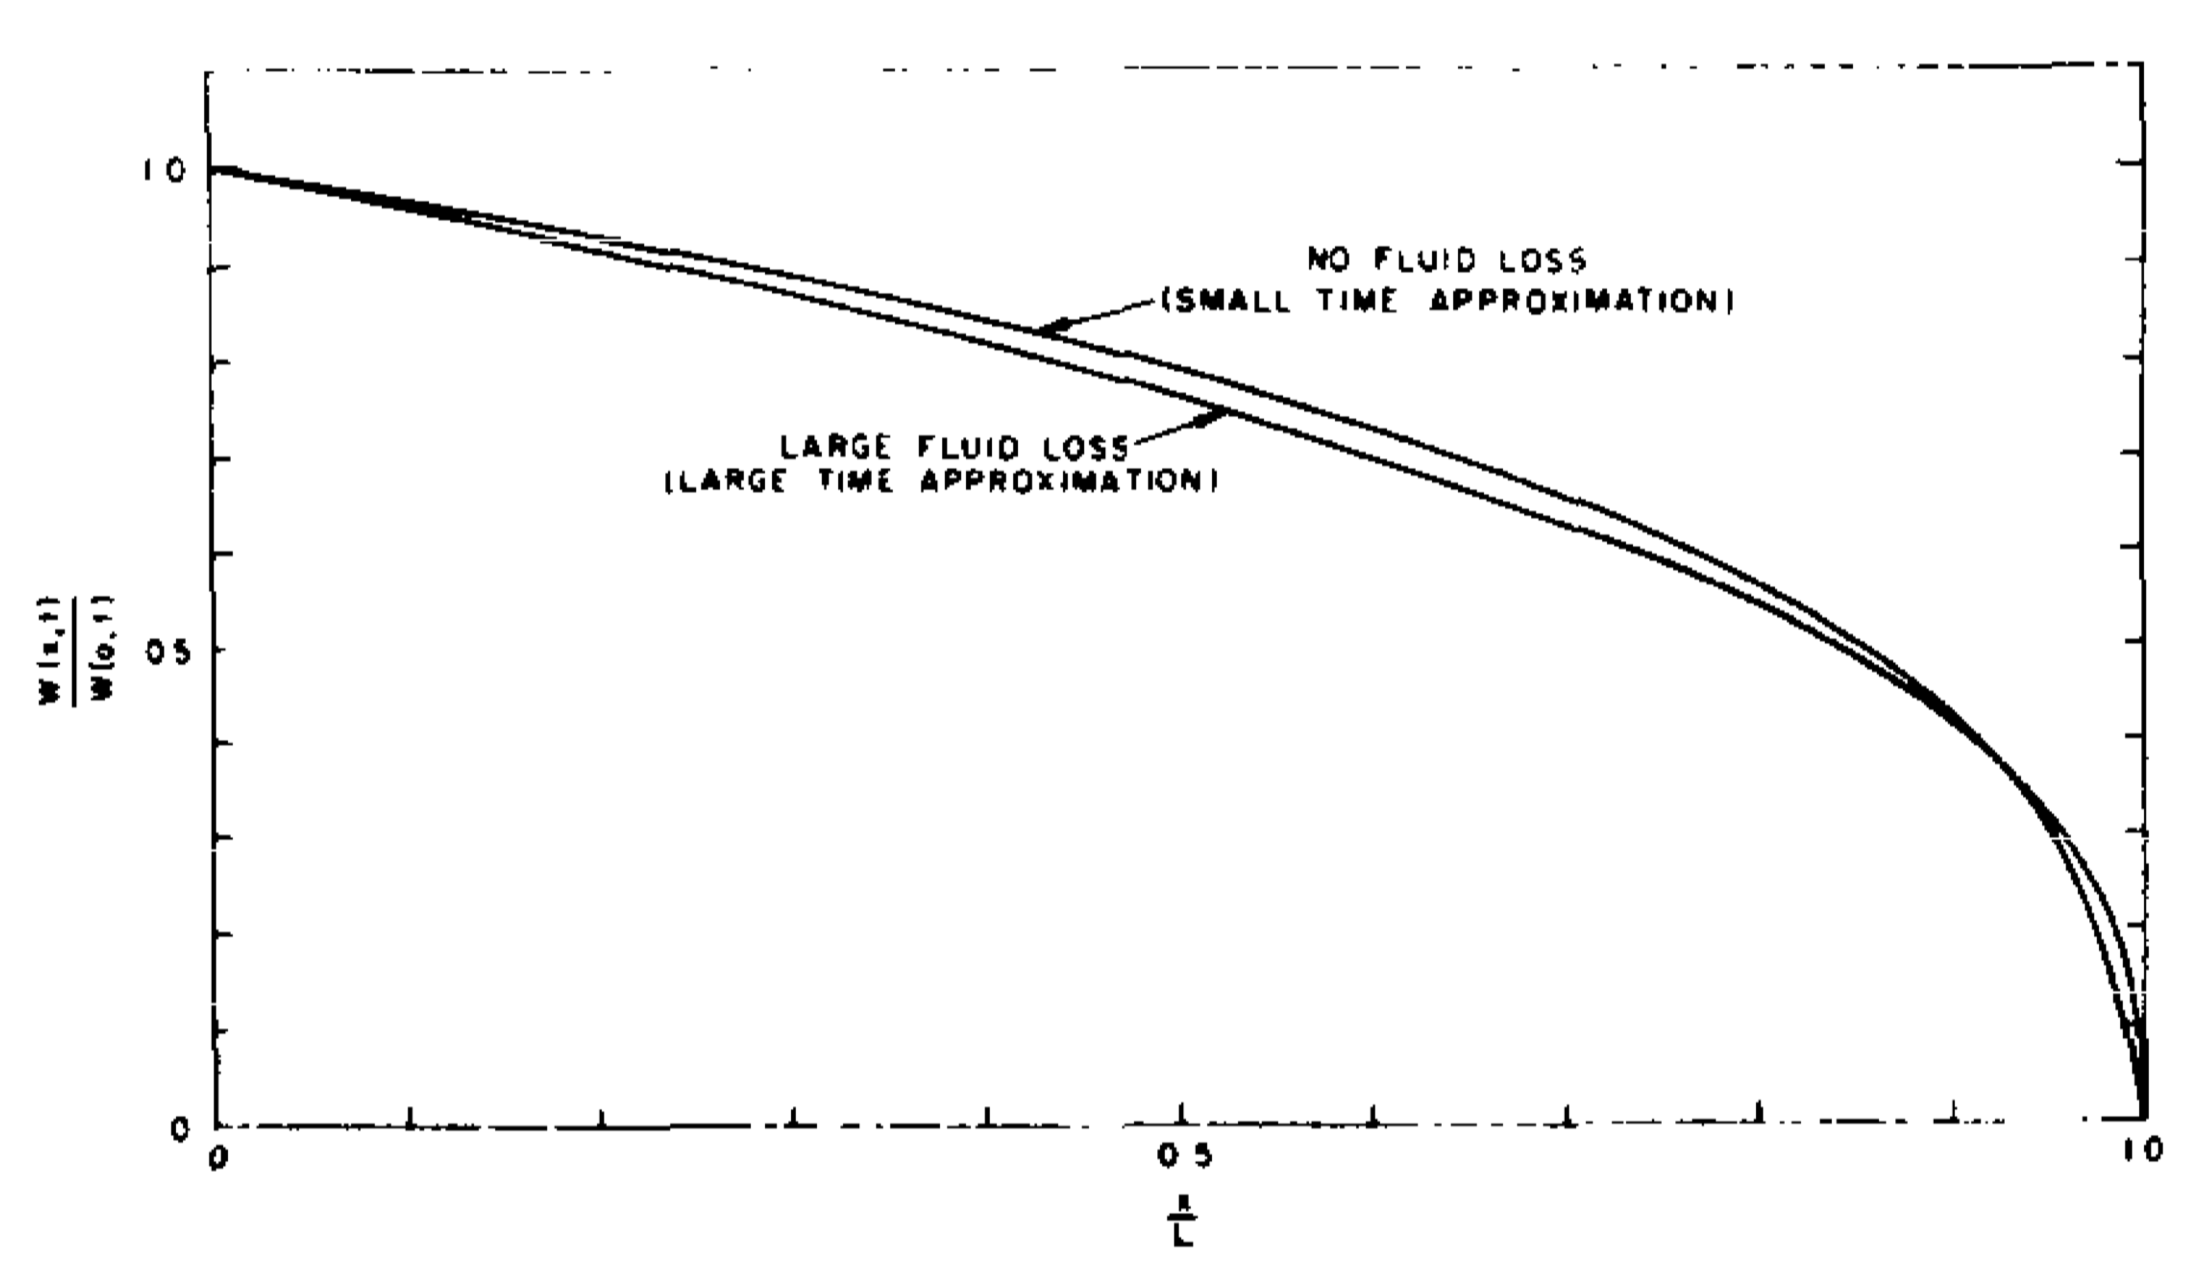
\includegraphics[width=0.8\textwidth]{maximum_width_vs_distance_from_well}
\caption{Максимальная безразмерная ширина трещины около скважины в зависимости от расстояния от скважины} 
\label{fig:width-vs-distance-from-well}
\end{figure}


Для любой конкретной задачи длину и ширину трещины в любой момент времени можно получить из рис. \ref{fig:length-vs-time}-\ref{fig:width-vs-distance-from-well} с помощью формул \eqref{Dimensionless}.
Можно просто вычислить значение $t_d$ из \eqref{Dimensionless}, найти $L_d(t_d)$ и $W_d(0,t_d)$ из рис.\ref{fig:length-vs-time} и \ref{fig:width-at-well-vs-time}, затем вычислить $L(t)$ и $W(0,t)$ из \eqref{Dimensionless}.
Затем примерное изменение максимальной ширины трещины по мере удаления от скважины следует из рис. \ref{fig:width-vs-distance-from-well}.
Кроме того, давление $\Delta p$ получается из $W$ по равенству \eqref{Max_W}.

Приближённые решения, представленные в приложениях B и C, дают существенное представление о влиянии физических параметров на длину, ширину и давление трещины.
Для случая большой скорости утечек или большого времени (Приложение B) длина трещины и максимальная ширина трещины около скважины определяются выражениями:
\beq\label{L_and_W_for_large_leak-off}
L(t)=\frac{q_i t^{1/2}}{\pi Ch}\,\,\,\,\,\,\,\,\,\,\,\,\,\,\,W(0,t)=4\left[\frac{2(1-\nu)\mu q_i^2}{\pi^3 GCh}\right]^{1/4}t^{1/8}
\eeq

Для случая отсутствия утечек или малого времени (Приложение C) эти же самые величины определяются выражениями:
\beq\label{L_and_W_without_leak-off}
L(t)=0.68\left[\frac{Gq_i^3}{(1-\nu)\mu h^4}\right]^{1/5}t^{4/5}\,\,\,\,\,\,\,\,\,\,\,\,\,\,\,W(0,t)=2.5\left[\frac{(1-\nu)\mu q_i^2}{Gh}\right]^{1/5}t^{1/5}
\eeq
Как видно из выражений \eqref{L_and_W_for_large_leak-off} и \eqref{L_and_W_without_leak-off} длина и ширина трещины растут быстрее со временем в случае отсутствия утечек (малое время), чем в случае больших утечек (большое время).
То, как другие параметры влияют на размер трещины, также видно из выражений \eqref{L_and_W_for_large_leak-off} и \eqref{L_and_W_without_leak-off}.
Например, $L$ пропорциональна $q_i$ в выражении \eqref{L_and_W_for_large_leak-off} и пропорциональна $q_i^{3/5}$ в выражении \eqref{L_and_W_without_leak-off}.
В выражении \eqref{L_and_W_for_large_leak-off} параметры $G$ и $\mu$ не влияют на длину $L$.

В приложении D проведено сравнение с приближённым решением Перкинса и Керна.
Установлено, что если выражения \eqref{L_and_W_for_large_leak-off} и \eqref{L_and_W_without_leak-off} свести к форме зависимостей $W(0,t)$ от $L$ (путём исключения времени $t$), то приближённое решение [6] довольно точно.
Тем не менее на ранних временах выражение \eqref{L_and_W_without_leak-off} для $L(t)$ отличается от формулы Картера [2], которая основана на предположении о постоянной ширине трещины.

На больших временах выражение \eqref{L_and_W_for_large_leak-off} для $L(t)$ согласуется с формулой Картера на больших временах [2], поскольку теперь доминирует эффект утечек жидкости в пласт.

Подробные исследования эффектов изменения параметров могут быть сделаны с помощью выражений \eqref{Dimensionless} и результатами на рисунках \ref{fig:length-vs-time} и \ref{fig:width-at-well-vs-time}, и эти исследования могут быть полезны при планировании дизайна ГРП.
Например, по этим результатам можно определить коэффициент утечек $C$, необходимый для достижения желаемой длины трещины после определённого времени закачки.
Можно определить давление закачки, необходимое для достижения желаемой скорости закачки.
Кроме того, трещина может быть спроектирована таким образом, чтобы раскрытие трещины пропускало проппант определённого размера.

Применяя изложенные выше результаты, необходимо иметь в виду основные предположения, сделанные при решении и постановке задачи.
Вероятно, наиболее важные предположения заключаются в том, что высота трещины ограничена по вертикали и что длина трещины намного больше высоты ($L\gg h$).
Как видно из рисунка \ref{fig:width-vs-distance-from-well}, последнее предположение обеспечивает медленное изменение ширины $w$ в зависимости от $x$, что подтверждает основное предположение о плоской деформации.
Если условие $L\gg h$, в частности сразу после образования трещины, не выполняется или если трещина не ограничена по вертикали, то более подходящими являются другие теоретические модели распространения трещины.
Для вертикальной трещины с $L\ll h$ и нагнетанием по всей высоте, модель плоской деформации в горизонтальной плоскости из [3,4,5] является более подходящей.
Если закачка ограничена коротким интервалом, то подходящей моделью должна быть радиально распространяющаяся вертикальная трещина, как предложили Перкинс и Керн [6].
Эта модель приблизительно была рассмотрена Гиртсмой, деКлерком [5] и другими.
Между решениями [3,4,5] и текущим решением есть существенные отличия.
В частности, для линейно распространяющейся (односторонней) вертикальной трещины приблизительная ширина трещины около скважины, данная Гиртсмой и деКлерком (для $\nu=0.25$), равна
$$
W(0)=2.1\left(\frac{\mu q_iL^2}{2Gh}\right)^{1/4},
$$
что отличается от нашего решения \eqref{L_and_W_for_large_leak-off} на больших временах на множитель $0.67\left(L/h\right)^{1/4}$.
Этот множитель велик, когда $L/h\ll1$ или $L/h\gg1$.
Как было сказано выше, наше решение неприменимо при $L/h<<1$.
С другой стороны, мы не считаем, что подход [3,4,5] верен при $L/h\gg 1$, поскольку предположение о вертикальной постоянной ширине в вертикальном направлении исключает смыкание трещины вверху и внизу.
Вносимая таким образом ошибка примерно пропорциональна $L$ и, таким образом, ошибка становится большой при $L\gg h$.
Напротив, ошибка, полученная в нашем решении с быстрыми изменениями вблизи кончика трещины примерно пропорциональна $h$, и эта ошибка становится малой при $L\gg h$.
Для $L\approx h$ необходимо трёхмерное решение, но в настоящее время оно отсутствует.
Такое решение также окончательно определило бы области применимости наших результатов и результатов работ [3,4,5].


\subsection{Список обозначений}
\setlength{\parindent}{0pt}
$A$ -- площадь поперечного сечения трещины\\
$C$ -- коэффициент утечек жидкости в пласт\\
$G$ -- объёмный модуль сдвига пласта\\
$h$ -- толщина пласта\\
$K$ -- константа (определяемая выражением \eqref{C-3})\\
$L$ -- длина трещины\\
$L_d$ -- безразмерная $L$\\
$p_f$ -- пластовое поровое давление\\
$q$ -- расход (объёмная скорость потока) жидкости через поперечное сечение трещины\\
$q_l$ -- скорость утечек на единицу длины трещины\\
$q_i$ -- постоянный расход жидкости в трещину на скважине\\
$S$ -- нормальное сжимающее напряжение плоскости трещины до гидроразрыва\\
$t$ -- время\\
$t_d$ -- безразмерное $t$\\
$u_l$ -- скорость утечек на единицу площади поверхности трещины\\
$v$ -- скорость жидкости\\
$W$ -- ширина трещины в центре трещины ($w_{max}$)\\
$W_d$ -- безразмерная $W$\\
$w$ -- ширина трещины\\
$x,y,z$ -- координаты в прямоугольной декартовой системе координат (рис. \ref{fig:kgd-model-geometry})\\
$x_d$ -- безразмерная координата $x$\\
$\Delta p$ -- давление в трещине минус $S$\\
$\mu$ -- вязкость жидкости гидроразрыва\\
$\nu$ -- объёмный коэффициент Пуассона пласта\\
$\tau(x)$ -- время начала утечек жидкости на расстоянии $x$ от скважины
\setlength{\parindent}{20pt}

\subsection{Список цитированной литературы}
\setlength{\parindent}{0pt}
[1] Howard, G.C. and Fast, C.R.: Hydraulic Fracturing, Monograph Series, Society of Petroleum Engineers, Dallas (1970) Vol. II.

[2] Carter, R.D.: "<Derivation of the General Equation for Estimating the Extent of the Fractured Area"> Appendix to: "<Optimum Fluid Characteristics for Fracture Extension"> by G. C. Howard and C. R. Fast, Drill. and Prod. Prac., API (1957) 261-270.

[3] Khristianovic, S.A. and Zheltov, Y.P.: "<Formation of Vertical Fractures by Means of Highly Viscous Liquid"> Proc., Fourth World Pet. Cong., Rome (1955) Sec. 2, 579-586.

[4] Baron, G. et al.: "<Fracturation hydraulique; bases the oriques, estudes de laboratorie, essais sur champ"> Proc., Seventh World Pet. Cong., Mexico City (1967) Sec. 3, 371.

[5] Geertsma, J. and de Klerk, F.: "<A Rapid Method of Predicting Width and Extent of Hydraulically Induced Fractures">, J. Pet. Tech. (Dec., 1969) 1571-1681.

[6] Perkins, T.K. and Kern, L.R.: "<Widths of Hydraulic Fractures">, J. Pet. Tech. (Sep., 1961) 937-949.

[7] Kern, L.R., Perkins, T.K and Wyant, R.E.: "<Designing Aluminum-Pellet Fracturing Treatments">, Drill. and Prod. Prac., API (1961).

[8] England, A.H. and Green, A.E.: "<Some Two-Dimensional Punch and Crack Problems in Classical Elasticity"> Proc., Cambridge Phil. Soc. (1963) Vol. 5, 489.

[9] Geertsma, J.: "<Problems of Rock Mechanics in Petroleum Engineering"> Proc., First Congress International Society of Rock Mechanics, Lisbon (1966) 585-594.

[10] Lamb, H.: Hydrodynamics, 6th Ed., Dover Publications, Inc., New York (1932).

[11] Hall C.D., Jr. and Dollarhide, F.E.: "<Performance of Fracturing Fluid Loss Agents Under Dynamic Conditions">, J. Pet. Tech. (July, 1968) 763-769.

[12] Ames, W.F.: Nonlinear Partial Differential Equations in Engineering, Academic Press, Inc., New York (1965).

\setlength{\parindent}{20pt}

\subsection{Приложение A. Численное решение}

Здесь мы получим конечно-разностный аналог уравнений \eqref{Initial_cond}-\eqref{GU_2} и дадим численный метод решения.
Чтобы получить конечно-разностные уравнения, удовлетворяющие общему условию баланса жидкости, начнём вывод с уравнения неразрывности \eqref{Continuity} вместе с выражениями \eqref{leak-offs}, \eqref{leak-off} и \eqref{gu1}, т.е.

\beq\label{A-1}
\frac{\partial q}{\partial x}+\frac{2hC}{\sqrt{t-\tau(x)}}+\frac{\partial A}{\partial t}=0,\,\,\,\,\,\,\,\,\,\,0<x<L
\tag{A-1}
\eeq

\beq\label{A-2}
q(0,t)=q_i
\tag{A-2}
\eeq

Интегрирование уравнения \eqref{A-1} по времени от $t_m$ до $t_{m+1}$ с использованием формулы трапеций даёт:
\beq\label{A-3}
\frac{\Delta t_m}{2}\frac{\partial}{\partial x}\left(q^{m+1}+q^m\right)+\left[4hC\sqrt{t-\tau(x)}+A\right]_{t_m}^{t_{m+1}}=0
\tag{A-3}
\eeq
где
$$
\Delta t_m=t_{m+1}-t_m\,\,\,\,\,,\,\,\,\,\,q^m=q(x,t_m).
$$

Интегрирование уравнения \eqref{A-3} по $x$ от $x_{i-1/2}$ до $x_{i+1/2}$ с использованием уравнения \eqref{A_area} и центрального значения для интеграла даёт:
\beq\label{A-4}
\frac{\Delta t_m}{2\Delta x}\left(q_{i+\frac{1}{2}}^{m+1}-q_{i-\frac{1}{2}}^{m+1}+q_{i+\frac{1}{2}}^{m}-q_{i-\frac{1}{2}}^{m}\right)+4hC\left(\sqrt{t_{m+1}-\tau_i}-\sqrt{t_m-\tau_{i}}\right)+\frac{\pi h}{4}\left(W_i^{m+1}-W_i^m\right)=0
\tag{A-4}
\eeq
где
$$
\Delta x=x_{i+\frac{1}{2}}-x_{i-\frac{1}{2}}\,\,\,,\,\,\,W_i^m=W(x_i,t_m)\,\,\,,\,\,\,x_i=\frac{1}{2}\left(x_{i+\frac{1}{2}}+x_{i-\frac{1}{2}}\right).
$$

Если мы примем $x_{\frac{1}{2}}=0$, то из уравнения \eqref{A-2}:
\beq\label{A-5}
q_{\frac{1}{2}}^m=q_i
\tag{A-5}
\eeq
и из уравнения \eqref{Continuity}:
\beq\label{A-6}
W_i^0=0
\tag{A-6}
\eeq

Конечно-разностный аналог уравнения \eqref{q_vs_w}:
\beq\label{A-7}
q_{i+\frac{1}{2}}=-\frac{\pi G}{256(1-\nu)\mu\Delta x}\left[\left(W_{i+1}^m\right)^4-\left(W_i^m\right)^4\right]
\tag{A-7}
\eeq

Результатом подстановки уравнения \eqref{A-7} в уравнение \eqref{A-4} является нелинейная система уравнений с неизвестным $W_i^{m+1}$ и с считаемым известным $W_i^m$.
Чтобы решить эту систему запишем:
\beq\label{A-8}
W_i^{m+1}=W_i^m+\Delta W_i^m
\tag{A-8}
\eeq
и примем, что
\beq\label{A-9}
\left(W_i^{m+1}\right)^4\approx\left(W_i^m\right)^4+4\left(W_i^m\right)^3\Delta W_i^m
\eeq

При подстановке уравнений \eqref{A-6}, \eqref{A-8} и \eqref{A-9} в уравнение \eqref{A-4} мы получим алгебраическую линейную трёхдиагональную систему уравнений, которая может быть просто решена для $\Delta W_i^m$ при $m=1,2,...$. 

\subsection{Приложение B. Решение при доминировании утечек жидкости}

\subsection{Приложение C. Решение при отсутствии утечек жидкости в пласт}

где
\beq\label{C-3}
K=\frac{G}{64(1-\nu)\mu h}
\tag{C-3}
\eeq

\subsection{Приложение D. Приближения Перкинса и Керна}

Для простоты сравнения мы записываем здесь приближенное решение Перкинса и Керна [6].

\beq
w=4\left[\frac{(1-\nu)\mu q_1L}{\pi G}\left(1-\frac{x}{L}\right)\right]^{1/4}
\eeq


\subsection{Приложение E. Влияние ступенчатых потерь на длину трещины}



\end{document}
